% Tipo de documento y tamaño de letra
\documentclass[letterpaper,10pt,twoside,onecolumn]{article}
\textwidth=15cm
% Preparando para documento en Español.
% Para documento en Inglés no hay que hacer esto.
\usepackage[spanish]{babel}
\usepackage{graphicx}
\selectlanguage{spanish}
\usepackage[utf8]{inputenc}
\begin{document}
 
\title{PRIMERA PRACTICA FORTRAN} 
\author{Ana Magdalena Sotomayor} 

\maketitle 
\section{INTRODUCCION}
Se codificaron 8 nuevos programas tales que realizan operaciones para obtener el area de un circulo, el volumen de un liquido dentro de una esfera, funciones trigonometricas, Comprobacion de la precision numerica del ordenador en 8 bits y 4 bits y los valores de diferentes funciones matematicas.

\section{CODIGOS} 
\subsection{Calcular el área de un circulo}
\begin{verbatim}
! Area . f90 : Calculates the area of a circle, sample program
 Program areacirculo ! Begin main program
  Implicit None ! Declare all variables
   Real *8 :: radius , circum , area ! Declare Reals
   Real *8 :: PI = 4.0 * atan(1.0) ! Declare , assign Real
  Integer :: model_n = 1 ! Declare , assign Ints
   print * , 'Enter a radius:' ! Talk to user
   read * , radius ! Read into radius
  circum = 2.00 * PI * radius ! Calc circumference
  area = radius * radius * PI ! Calc area
  print * , 'Program number =' , model_n ! Print program number
  print * , 'Radius =' , radius ! Print radius
  print * , 'Circumference =' , circum ! Print circumference
  print * , 'Area =' , area ! Print area
 End Program areacirculo ! End main program code
\end{verbatim}

\subsection{Imagen de salida}
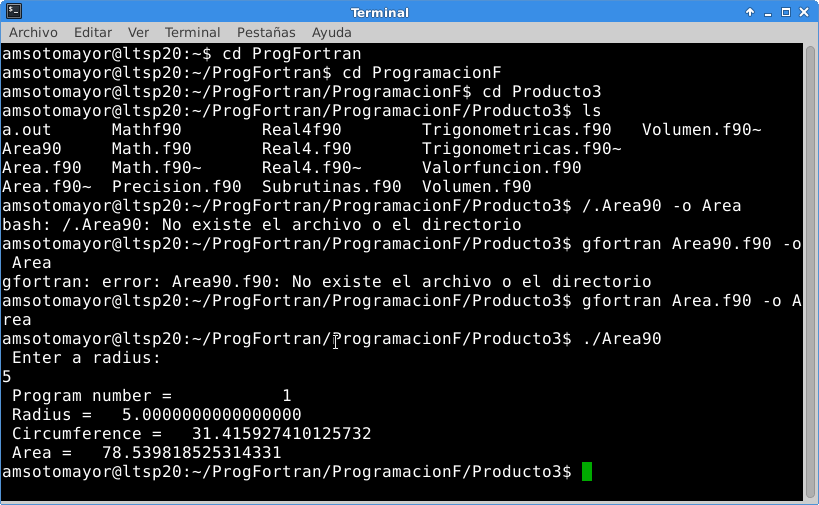
\includegraphics[scale=.50]{Area.png}

\subsection{Calculos Matematicos}
\begin{verbatim} ! Math . f90 : demo some Fortran math functions
  Program Math2! Begin main program

   Complex *8 :: x=- 1.0 , y=2, z=0 ! Declare variables x, y, z
  x = sqrt (x)  
  y = asin (y) ! Call the sine function
  z = log (z) ! Call the exponential function
  print * , x, y, z ! Print x, y, z
 End Program Math2 ! End main program
\end{verbatim}
\subsection{Imagen de salida}
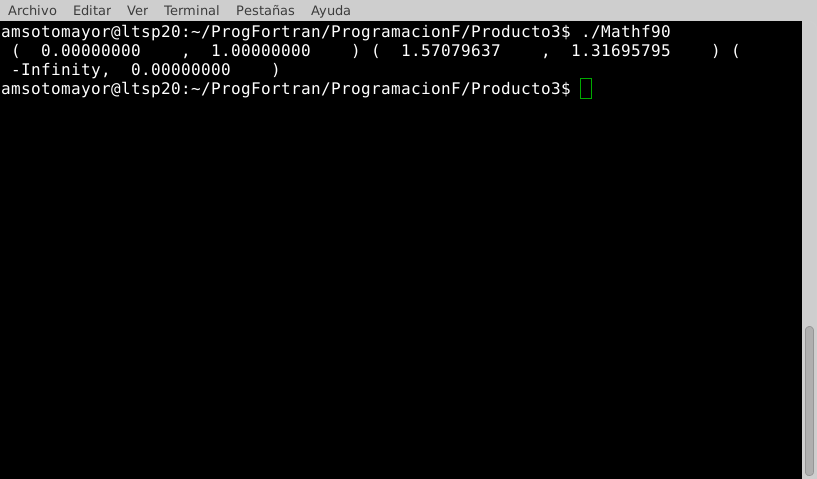
\includegraphics[scale=.75]{Math.png}

\subsection{Precision del Ordenador con numeros Reales en 8 bits}
\begin{verbatim}
! Limits . f90 : Determines machine precision
 Program Limits
   Implicit None
   Integer :: i , n
   Real *8 :: epsilon_m , one
   n=60 ! Establish the number of iterations
   ! Set initial values :
   epsilon_m = 1.0
  one = 1.0
  ! Within a DO-LOOP, calculate each step and print .
  ! This loop will execute 60 times in a row as i is
  ! incremented from 1 to n ( since n = 60) :

  do i = 1, n , 1 ! Begin the do-loop
    epsilon_m = epsilon_m / 2.0 ! Reduce epsilon m
    one = 1.0 + epsilon_m ! Re-calculate one
    print * , i , one , epsilon_m ! Print values so far
  end do ! End loop when i>n
 End Program Limits 
\end{verbatim}
\subsection{Imagen de salida}
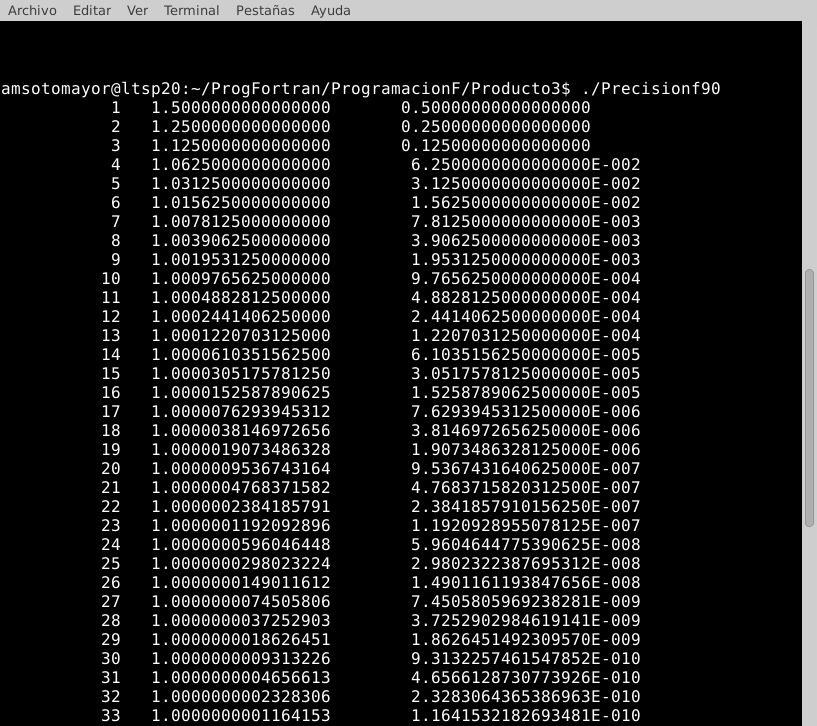
\includegraphics[scale=.75]{Precision.png}

\subsection{Programacion de Precision del ordenador en 4 bits}
\begin{verbatim}
! Limits . f90 : Determines machine precision
! LOOP, calculate each step and print .
 ! This loop will execute 60 times in a row as i is
 ! incremented from 1 to n ( since n = 60) :

 do i = 1, n , 1 ! Begin the docalculate one
   print * , i , one , epsilon_m ! Print values so far
 end do ! End loop when i>n
End Program Real4 
\end{verbatim}
\subsection{Imagen de salida}
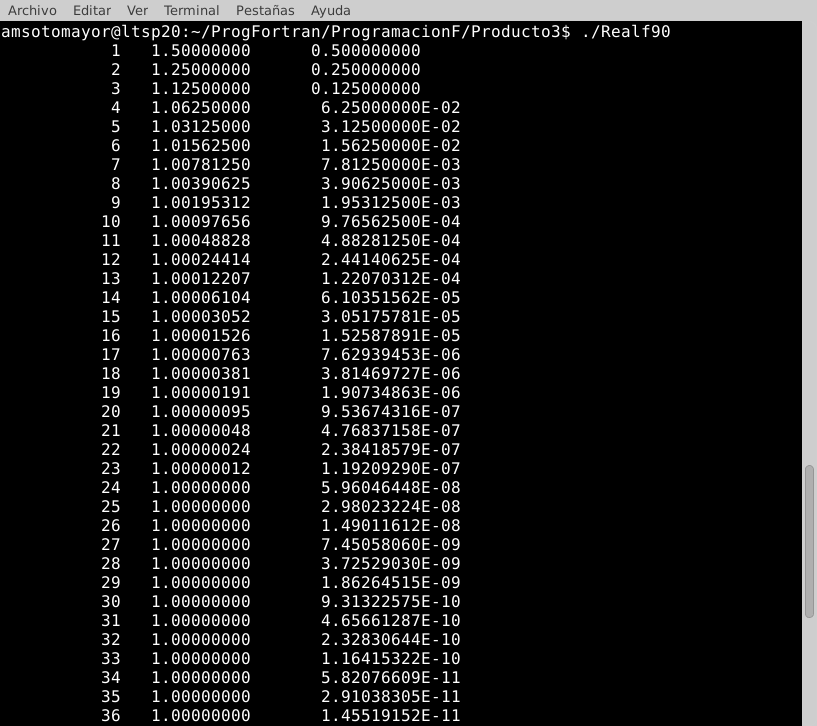
\includegraphics[scale=.75]{Real4.png}

\subsection{Subrutinas}
\begin{verbatim}
! Subroutine . f90 : Demonstrates the call for a simple subroutine
 ! ---------------------------------------------
 Subroutine g(x, y, ans1 , ans2 )
   Implicit None
   Real (8) :: x , y , ans1 , ans2 ! Declare variables
   ans1 = sin (x*y) + 1. ! Use sine intrinsic func.
   ans2 = ans1**2
 End Subroutine g
 !
 Program Mainprogram ! Demos the CALL
   Implicit None
   Real *8 :: Xin =0.25 , Yin =2.0 , Gout1 , Gout2
   call g( Xin , Yin , Gout1 , Gout2 ) ! Call the subr g
   write ( * , *) 'The answers are: ' , Gout1 , Gout2
End Program Mainprogram 
\end{verbatim}     
\subsection{Imagen de salida}
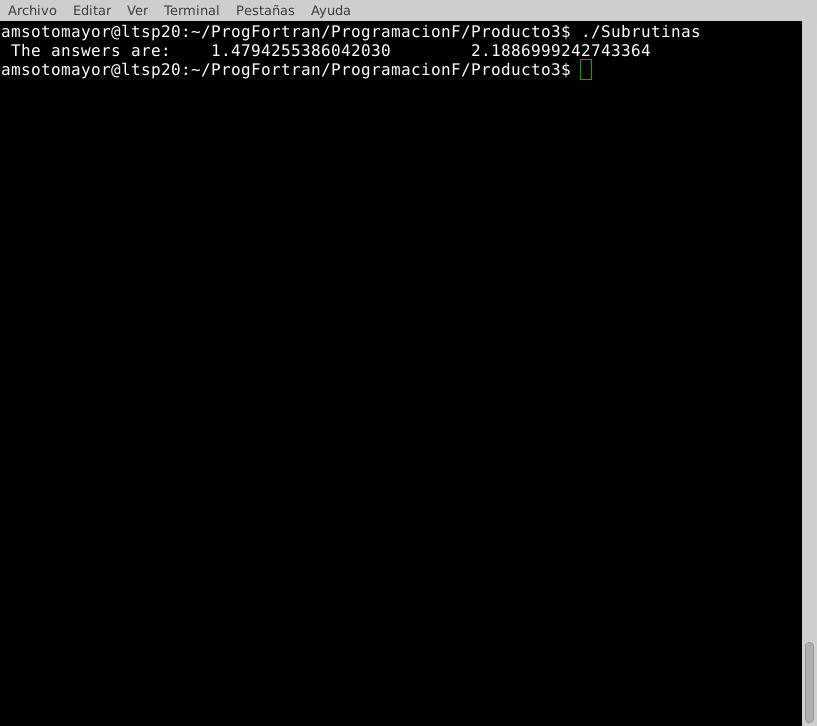
\includegraphics[scale=.75]{Subrutinas.png}

\subsection{Funciones Trigonometricas}
\begin{verbatim}
! Math . f90 : demo some Fortran math functions
! 
Program Mathtest! Begin main program

  Real *8 :: x = 1.0 , y, z ! Declare variables x, y, z
  y = sin (x) ! Call the sine function
 z = exp (x) + 1.0 ! Call the exponential function
 print * , x, y, z ! Print x, y, z
End Program Mathtest ! End main program 
\end{verbatim}
\subsection{Imagen de salida}
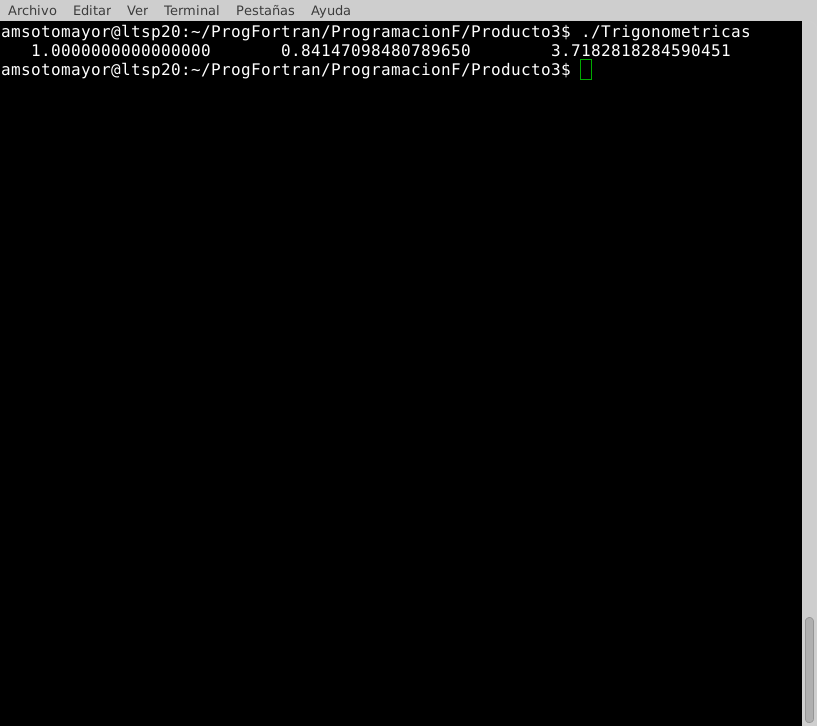
\includegraphics[scale=.75]{Trigonometricas.png}

\subsection{El Valor de una funcion dada}
\begin{verbatim}
 ! Function . f90 : Program calls a simple function
 ! -------------------------------
 Real *8 Function f (x,y)
   Implicit None
   Real *8 :: x, y
   f = 1.0 + sin (x*y )
 End Function f
 !
 Program Main
  Implicit None 
  Real *8 :: Xin =0.25 , Yin =2. , c , f ! declarations ( also f)
  c = f ( Xin , Yin )
  write ( * , * ) 'f(Xin, Yin) = ' , c
 End Program Main 
\end{verbatim}
\subsection{Imagen de salida}
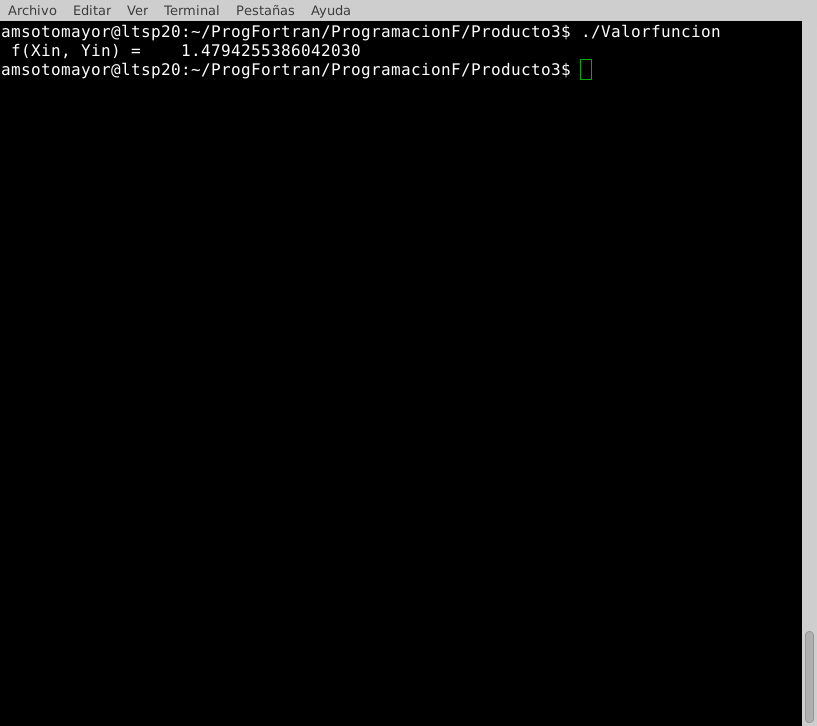
\includegraphics[scale=.75]{Valorfuncion.png}

\subsection{Volumen de un liquido en una esfera}
\begin{verbatim}
! Area . f90 : Calcular el volumen de liquido en un tanque esferico
 ! -----------------------------------------------
 Program Sphere_volume ! Begin main program
  Implicit None ! Declare all variables
   Real *8 :: radius , height , volume , Newradius ! Declare Reals
   Real *8 :: PI = 4.0 * atan(1.0) ! Declare , assign Real
  Integer :: model_n = 1 ! Declare , assign Ints
   print * , 'Enter a radius:' ! Talk to user
   read * , radius ! Read into radius
   print * , 'Enter a height:' ! Talk to user
   read * , height ! Tomar el valor de la h
   Newradius =  3 * radius - height  ! Calc volume
   volume = 0.3333 * PI * height * height * Newradius
 print * , 'Program number =' , model_n ! Print program number
  print * , 'Radius =' , radius ! Print radius
  print * , 'height =' , height ! Print height
  print * , 'Volume =' , volume ! Print circumference
 End Program Sphere_volume ! End main program code
\end{verbatim}
\subsection{Imagen de salida}
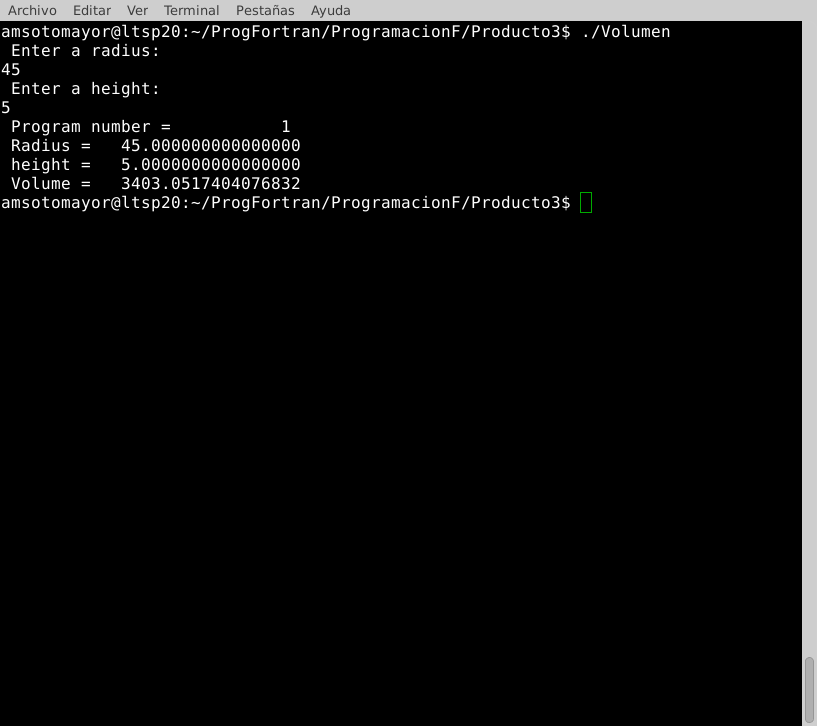
\includegraphics[scale=.75]{Volumen.png}

% Nunca debe faltar esta ultima linea.
\end{document}